% !TeX spellcheck = en_GB
\chapter{Secondary Objectives}
\section{API for BSI Catalog - Priority: LOW}
The application programming interface (API) should offer straightforward REST access to read, create, edit and possibly manage the content of the wiki heeding the permission settings in place.
This includes the News section, tutorials as well as the BSI catalogue itself.
Such access could be used for a future integration into a mobile application.
Existing wiki-frameworks might already include ready-to-use API functionalities and could be used.


\section{FAQ - Priority: MEDIUM}



\begin{tcolorbox}[breakable,colback=red!14,colframe=red!40!black,title=UPDATE 19/11/2017]
The website should have an page showing Frequently Asked Questions (FAQ) and there answers.
Questions should be grouped by theme and answers hidden behind expandable questions. 
This gives the guest a better overview on the questions that are dealt with.
The FAQ should be accessible through the bottom section and should also be present on the tutorial overview page.
Content will be provided by the analysis team.
\end{tcolorbox}


\section{Forum (Work in Progress) - Priority: MEDIUM}



\section{Labels - Priority: HIGH}
 
\begin{tcolorbox}[breakable,colback=red!14,colframe=red!40!black,title=UPDATE 30/11/2017]
Labels should inform website users about the current state of content. 
\\
Types of labels:
\begin{itemize}
    \item creation status: an automatically generated label which gives information about how long ago the content has been created\\
Formatting in hours, weeks, months and years
    \item unchecked/checked:The default is unchecked, content read by moderators and where the content is appropriate will get a checked label
    \item helpful label: For a certain number of upvotes, content should get a helpful label\\
this should be scalable
    \item content type: use labels as a 'path'/show where the page is: news, archive, BSIc\\
several content types possible
\end{itemize}

It should be possible to label each content, articles as well as news.


\end{tcolorbox}

Here are some examples for label
\begin{figure}[h] 
    \centering
    
\includegraphics[scale=1.0]{Pictures/label1}
    \caption{Waffle label analyse}
\end{figure} 
\begin{figure}[h] 
    \centering
    
\includegraphics[scale=1.0]{Pictures/label2}
    \caption{Waffle label programming}
\end{figure}

\section{Up/Down Votes - Priority: HIGH}
\begin{tcolorbox}[breakable,colback=red!14,colframe=red!40!black,title=UPDATE 30/11/2017]
Article votes would be nice in form of a “Did find this this article helpful?” Question with yes/no buttons at the end of it, which could generate after a few yes a label “Helpful”.
Every website user can vote, including the guest.
\end{tcolorbox}

\section{Reputation Points (Karma Points) - Priority: MEDIUM}
\begin{tcolorbox}[breakable,colback=red!14,colframe=red!40!black,title=UPDATE 30/11/2017]
Reputation points should motivate users to get involved on the side and reward them for that.\\
\end{tcolorbox}
\begin{figure}[!tbp]
  \centering
\begin{minipage}[b]{0.6\textwidth}
    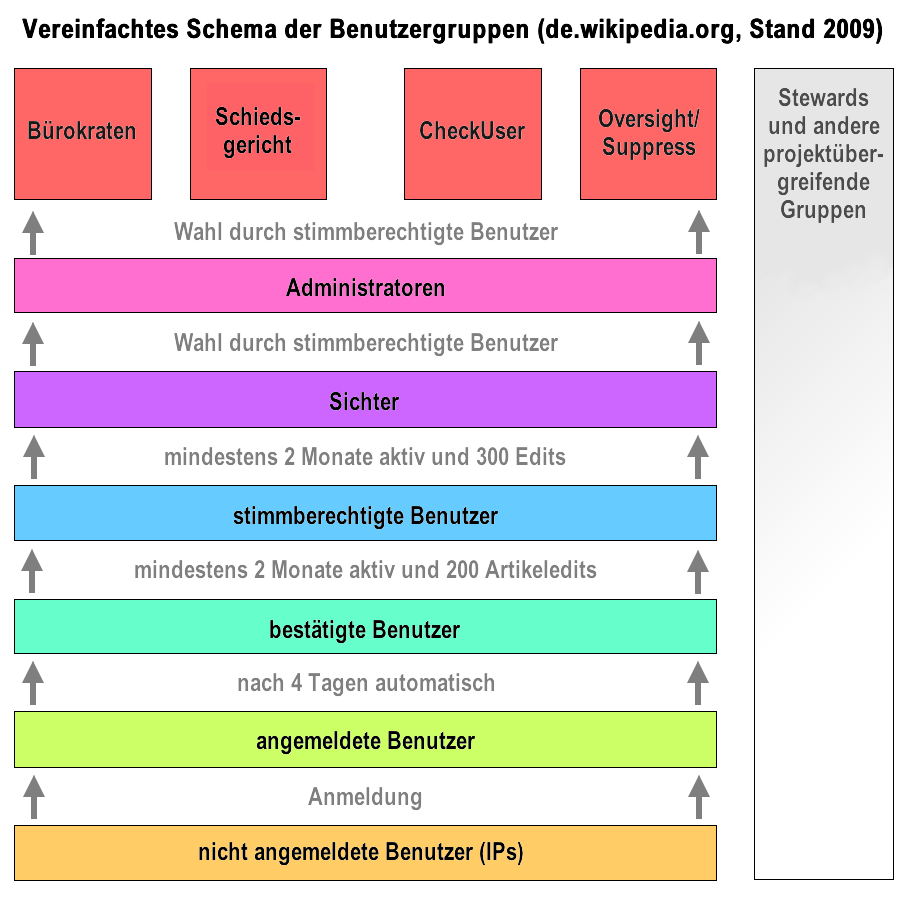
\includegraphics[width=\textwidth]{Pictures/Wikipedia}
    \caption{Wikipedia User Structure}
  \end{minipage}
  \hfill
  \begin{minipage}[b]{0.3\textwidth}
    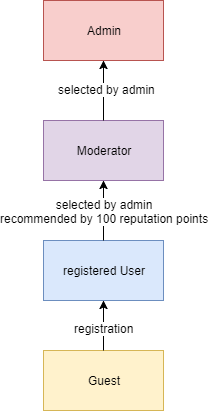
\includegraphics[width=\textwidth]{Pictures/UserStructure}
    \caption{our User Structure}
  \end{minipage}
\end{figure}

\begin{tcolorbox}[breakable,colback=red!14,colframe=red!40!black,title=UPDATE 30/11/2017]
We would like to keep a similiar (best-practice) user structure to Wikipedia. In our system we will have admins, the “sichter” will be our “moderator”, we will also have registered user and guests. \\
However after intensive discussion about how Karma (or reputation points) is generated, we decided to just keep the “article upvoting” generated votes for an article only without passing it to the user, since the quality of writing / editing, perhaps only a few, article isn’t representative of the trustworthiness of a user.\\
Only users which have had a big number (100) of approved edits/writings can become a mod and edit articles without being reviewed, or review other people. 
\end{tcolorbox}


\section{User Access to BSI Catalogue Pages - Priority: HIGH}
\label{2nd_bsi_link}
While the general access to alter the pages of the BSI catalogue should be restrictive (see section~\ref{BSIc}) users who write an article should still be allowed to link their article in the pages of the BSI catalogue.


\section{Automatically created best 10 suggestions when linking to bsi- Priority: LOW}
\begin{tcolorbox}[breakable,colback=red!14,colframe=red!40!black,title=UPDATE 01/12/2017]
   For mockups of the linking process detailled here see Appendix~\ref{appendix_bsi_link}.
   The best 10 Suggestions are nice to have but low periorized. It would be nice if these suggestions appear automatically after writing an article. Our idea was that these suggestions would be found through the internal search. These suggestions are always updated when the user enters something again in the search field. This topic is low-periodized and does not need to be strongly considered.   
\end{tcolorbox}


\begin{tcolorbox}[breakable,colback=red!12,colframe=red!40!black,title=UPDATE 15/11/2017]
    For mockups of the linking process detailled here see Appendix~\ref{appendix_bsi_link}.
    After or while users write their articles they are presented with the option to link it to the BSI catalogue.
    This option leads users to another page. Here:
    \begin{itemize}
            \begin{comment}
        \item on their first visit, users are presented with 
            \end{comment} 
        \item users can search for wiki content they want to link to,
        \item users can directly browse the BSI tree to find the page they want to link to,
        \item on the left  users see a list of titles of wiki pages that they already have linked their article to
            .
    \end{itemize}
    There is no restriction on the number of pages an article can be linked to.
    So the list of linked pages should offer a scroll bar if the list exceeds the page limits.
    If users click on a search result, a BSI tree item or an item of the list of linked to wiki pages they are brought to the page in question.
    There, if users want to link to a word they click on/mark the word they want to link their article to.
    Alternatively, they click on/mark the ``See also'' section of the page.
    Both times the selection has to be confirmed and brings the user back to the second page which features the list of linked pages.
    The list of search results should be limited to ten.
    So that, users have to change or add to his keywords if they did not get the page they were looking for.
    All pages should have a ``Back'' or ``Cancel'' button.  
\end{tcolorbox}





\section{Automatically archiving News (Work in Progress) - Priority: LOW}



\section{Automatically publishing User News without Approval (Work in Progress) - Priority: LOW}



\section{One Sentence News (Work in Progress) - Priority: LOW}



\section{Archiving old Articles (Work in Progress) - Priority: MEDIUM}
\subsection{User Prompt to relink Article (Work in Progress)}

\subsection{Auto-Archiving}
\label{archive_relcon}
Related content to a BSI catalogue version refers to wiki content created by users which is obsolete with the new catalogue version. 
An indicator for the obsolescence is that during a BSI catalogue update the article is only linked to the current catalogue but will not get relinked to the new version.


\section{Extended Wizard (Work in Progress) - Priority: LOW}

